\section{\'Equipement}

\subsection{Armures}
Voici quelques armure que l'on peu trouver dans l'univers de \swfe. Il s'agit là plus d'une grille d'étalonnage que d'une liste exhaustive. La limite c'est l'imagination des joueurs et la volonté du MJ.

\begin{dnditemtable}[ l c c c ]
    \textbf{Type} & \textbf{Armure} & \textbf{Poids} & \textbf{Prix} \\
    Veste en Cuir           & +1  & 10 & 50        \\
    Casque                  & +4  &  5 & 80        \\
    Armure Storm Trooper    & +6  & 20 & Militaire \\
    Armure mandalorienne    & +7  & 15 & 1000      \\
    M'uhk'gla (lourde)      & +14 & 30 & 2500      
\end{dnditemtable}

\begin{center}
	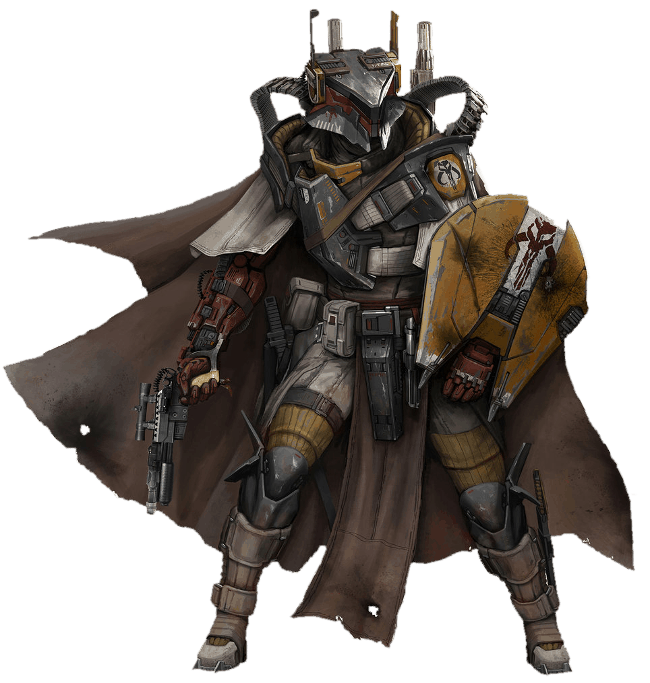
\includegraphics[width=\linewidth]{img/equipement/mandalorian_heavy_armor.png}
	\caption{\emph{Armure lourde Mandalorienne}}
\end{center}

\subsection{Armes}

\subsubsection{Combat corps à corps}

\begin{dnditemtable}[ l c c c ]
    \textbf{Type} & \textbf{Dégats} & \textbf{Poids} & \textbf{Prix} \\
    Vibrolame				& For+d4    &  1 & 25		 \\
    Bâton           		& For+d4    &  1 & 10        \\
    Couteau laser			& 2d6+4     &  1 & 500		 \\
    Vibroépée				& For+d6+2  &  6 & 250		 \\
    Bâton électrique        & For+d8+2  & 10 & 700	
\end{dnditemtable}

\subsubsection{A distance}

\clearpage
\subsection{Armes Spéciales}

\subsubsection{Sabre Laser}
\label{sec:sabre-laser}

\begin{flushright}
	\vspace{-5\baselineskip}
	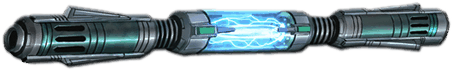
\includegraphics[width=5cm, angle=-25]{img/equipement/lightsaber01.png}
	\vspace{-1\baselineskip}
\end{flushright}

Le sabre laser est l'arme des chevaliers combattant avec la Force, qu'ils soient du Côté Obscur ou du Côté Lumineux. La lame est un faisceau d'énergie pure, produit par généralement trois cristaux polis contenus dans le manche. Seuls les utilisateurs de la Force ont la compétence nécessaire pour l'utiliser. Tout autre utilisateur aurait autant de chances de se blesser que de blesser ses adversaires. 

Il existe une multitude de cristaux à travers la Galaxie, mais seuls certains d'entres eux, assez rigides, ou bien parfaitement constitués, peuvent être utilisés, et c'est selon les types des cristaux, que la lame arborera une certaine teinte. Chaque cristal peut receler un pouvoir lorsqu'il est alimenté. A travers les âges, beaucoup de ces cristaux furent découverts mais ils sont très rares et difficiles à déceler. En voici quelques exemples : cristal de Solari, cristal Damind, cristal Kaiburr, \ldots

Mais les Jedi arrivèrent également à créer des cristaux industriellement pour alimenter leurs besoins. Ces cristaux peuvent être modifiés lors de leur croissance pour avoir une lame de la couleur voulue, mais toutes les couleurs ne sont pas disponibles. Ces cristaux sont toutefois moins maniables, mais plus puissants que les cristaux naturels qui sont, à l'inverse, plus maniables mais moins puissants. Ce sont, en général, les Sith et les Jedi Noirs qui utilisent ce type de cristaux car ils recherchent la puissance, et non la maniabilité. Historiquement, les Sith ont toujours préféré des lames de couleur rouge. 

Le Sabre laser est une arme très rare, chaque Jedi fabrique le sien et il est unique. Il n'existe doc que deux façons de s'en procurer un, le fabriquer ou le volé sur le cadavre d'un Jedi.

La fabrication d'un Sabre laser n'est pas aisé:
\begin{enumerate}
	\item Trouvé tous les composants, une cellule d'énergie, une lentille, un émetteur de lame et un cristal.
	\item Apprendre les rudiment du montage d'un sabre (Connaissance (Jedi) d6+).
	\item Maîtriser la Force suffisement pour assaiblé les différentes pièce (Maîtrise de la Force d6+).
\end{enumerate}

Une fois toutes les conditions remplies, le Jedi dont méditer pendant un mois pour assembler les pièces de son sabre. Quand le sabre est terminé, lors de sa première utilisation, le joueur fait un jet de Maîtrise de la Force, s'il fait 1, le sabre explose, le composant sont perdu et le héro prend un niveau de blessure. Il faudra tout recommencer.

\newpage
\begin{center}
	\vspace*{\fill}
	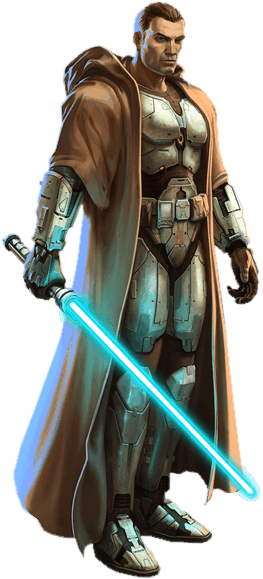
\includegraphics[width=0.7\linewidth]{img/equipement/jedi01.png}
	\vspace*{\fill}
\end{center}